\documentclass[a4paper]{scrartcl}
\usepackage{scrpage2}
\usepackage[ngerman]{babel}
\usepackage[T1]{fontenc}
\usepackage[utf8]{inputenc}
%\usepackage[pdftex]{graphicx}
%\usepackage[intlimits]{amsmath}
%\usepackage{listings}
%\lstset{frame=single,breaklines=true}
\usepackage{ amssymb }
\usepackage{amsmath}
\usepackage{hyperref}
\usepackage{enumerate}
\usepackage[a4paper, total={19cm, 23cm}]{geometry}
\usepackage{stmaryrd}
\usepackage{graphicx}
\pagestyle{scrheadings}
\pagenumbering{gobble}
\ihead{Übungsblatt 3\\Nils Werner 108012219293}
\chead{\\Paul Rösler 108012225686	}
\ohead{Übungsgruppe: Mo. 16:00\\Daniel Teuchert 108012214552}
\setheadsepline{0.4pt}
\begin{document}

\section*{Aufgabe 1}
Zu zeigen: $\{nor, c\}$ ist universell, zeige: $nand$ kann durch $nor$ dargestellt werden, da $\{nand,c\}$ universell ist (siehe Vorlesung), ist dann auch $\{nor, c\}$ universell.

\begin{figure}[htp] \centering{
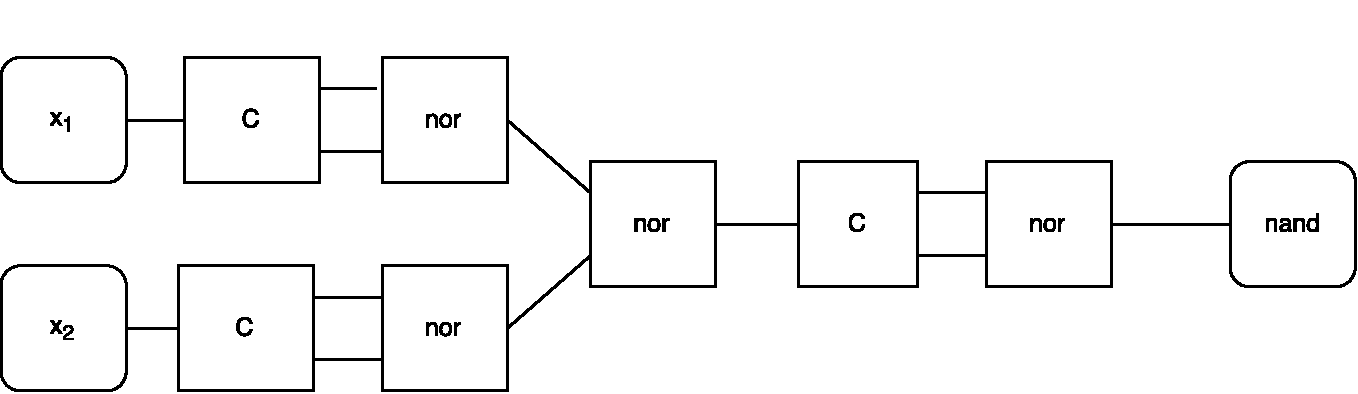
\includegraphics[scale=0.5]{nand.pdf}}
\caption{Schaltkreis $nand$ aus $nor$}
\end{figure}

$nand = \overline{\overline{\overline{x_1 \vee x_1} \vee \overline{x_2 \vee x_2}}~~\vee ~~\overline{\overline{x_1 \vee x_1} \vee \overline{x_2 \vee x_2}}}$\\
$= \overline{\overline{\overline{x_1} \vee \overline{x_2}}~~\vee ~~\overline{\overline{x_1} \vee \overline{x_2}}}$\\
$= \overline{(x_1 \wedge x_2)~~\vee ~~(x_1 \wedge x_2)}$\\
$= \overline{x_1 \wedge x_2}~~\wedge ~~\overline{x_1 \wedge x_2}$\\
$= \overline{x_1 \wedge x_2} = nand(x_1,x_2)$

\newpage
\section*{Aufgabe 2}

\begin{figure}[htp] \centering{
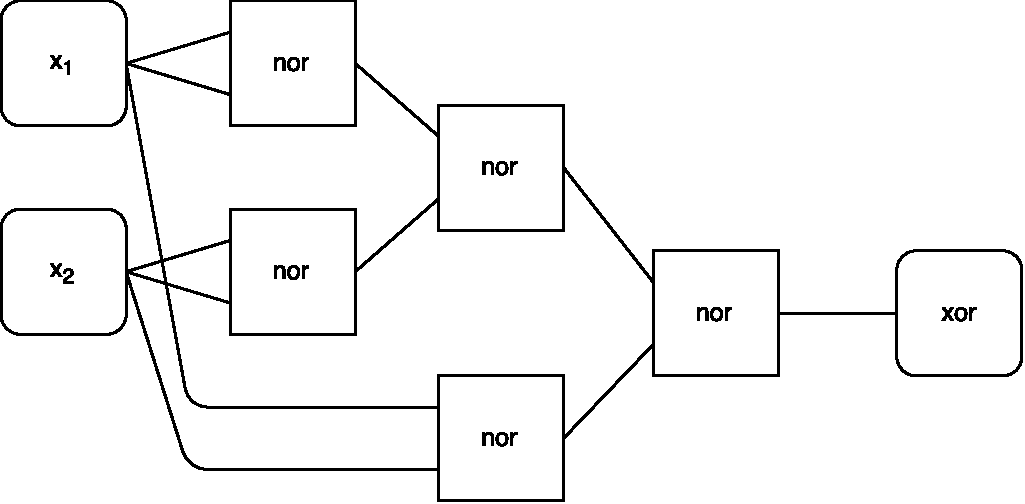
\includegraphics[scale=0.5]{xor.pdf}}
\caption{Schaltkreis $xor$ aus $nor$}
\end{figure}

\newpage
\section*{Aufgabe 3}

\newpage
\section*{Aufgabe 4}

\end{document}
